\documentclass{article}
\usepackage{amssymb}
\usepackage{mathtools}
\usepackage{amsmath}
\usepackage{hyperref}
\usepackage{setspace}
\usepackage[utf8]{inputenc}
 
\usepackage{listings}
\usepackage{color}
\usepackage{graphicx}
\usepackage[english]{babel}
 
\setlength{\parindent}{4em}
\setlength{\parskip}{1em}
 
\definecolor{codegreen}{rgb}{0,0.6,0}
\definecolor{codegray}{rgb}{0.5,0.5,0.5}
\definecolor{codepurple}{rgb}{0.58,0,0.82}
\definecolor{backcolour}{rgb}{0.95,0.95,0.92}
 
\lstdefinestyle{mystyle}{
    backgroundcolor=\color{backcolour},   
    commentstyle=\color{codegreen},
    keywordstyle=\color{magenta},
    numberstyle=\tiny\color{codegray},
    stringstyle=\color{codepurple},
    basicstyle=\footnotesize,
    breakatwhitespace=false,         
    breaklines=true,                 
    captionpos=b,                    
    keepspaces=true,                 
    numbers=left,                    
    numbersep=5pt,                  
    showspaces=false,                
    showstringspaces=false,
    showtabs=false,                  
    tabsize=2
}

\newcommand{\norm}[1]{\left\lVert#1\right\rVert}
 
\lstset{style=mystyle}

\everymath{\displaystyle}

\begin{document}

\raggedright

\doublespacing


\title{ {\Huge{Data Mining 2015 - Homework 3}} }
\author {Ludovico Fabbri 1197400}
\maketitle


\section{Problem 1}
For this exercise we will implement some versions of the A-priori algorithm.

Source code and output text files for this problem are located in the \textit{problem1} folder. All the questions of the problem are computed and solved in the \textit{program.py} file.
Below is the output:

\begin{lstlisting} 
/home/ludovicofabbri/anaconda/bin/python2.7 /home/ludovicofabbri/PycharmProjects/Homework3.2/program.py
SIMPLE APRIORI ON retail.dat
START
Round k = 1 Found 185 frequent itemsets
Round k = 2 Found 191 frequent itemsets
Round k = 3 Found 79 frequent itemsets
Round k = 4 Found 13 frequent itemsets
Round k = 5 Found 0 frequent itemsets
Found 468 frequent itemsets
TIME END: 2.12692284584

RANDOM APRIORI ON retail.dat, threshold = t * p = 50
START
Round k = 1 Found 194 frequent itemsets
Round k = 2 Found 192 frequent itemsets
Round k = 3 Found 87 frequent itemsets
Round k = 4 Found 16 frequent itemsets
Round k = 5 Found 0 frequent itemsets
Found 489 frequent itemsets with false positives
Found 429 frequent itemsets without false positives
False positives removed: 60
TIME END: 7.63972496986

RANDOM APRIORI ON retail.dat, threshold = t * p * 0.9 = 45
START
Round k = 1 Found 226 frequent itemsets
Round k = 2 Found 224 frequent itemsets
Round k = 3 Found 94 frequent itemsets
Round k = 4 Found 17 frequent itemsets
Round k = 5 Found 1 frequent itemsets
Round k = 6 Found 0 frequent itemsets
Found 562 frequent itemsets with false positives
Found 453 frequent itemsets without false positives
False positives removed: 109
TIME END: 8.7128610611

SIMPLE APRIORI ON webdocs.dat
START
Round k = 1 Found 22 frequent itemsets
Round k = 2 Found 65 frequent itemsets
Round k = 3 Found 64 frequent itemsets
Round k = 4 Found 29 frequent itemsets
Round k = 5 Found 6 frequent itemsets
Round k = 6 Found 0 frequent itemsets
Found 186 frequent itemsets
TIME END: 1182.52232099

RANDOM APRIORI ON webdocs.dat, threshold = t * p = 50
START
Round k = 1 Found 24 frequent itemsets
Round k = 2 Found 77 frequent itemsets
Round k = 3 Found 108 frequent itemsets
Round k = 4 Found 75 frequent itemsets
Round k = 5 Found 23 frequent itemsets
Round k = 6 Found 2 frequent itemsets
Round k = 7 Found 0 frequent itemsets
Found 309 frequent itemsets with false positives
Found 183 frequent itemsets without false positives
False positives removed: 126
TIME END: 185.007380009

RANDOM APRIORI ON webdocs.dat, threshold = t * p * 0.9 = 45
START
Round k = 1 Found 35 frequent itemsets
Round k = 2 Found 135 frequent itemsets
Round k = 3 Found 203 frequent itemsets
Round k = 4 Found 157 frequent itemsets
Round k = 5 Found 64 frequent itemsets
Round k = 6 Found 11 frequent itemsets
Round k = 7 Found 0 frequent itemsets
Found 605 frequent itemsets with false positives
Found 186 frequent itemsets without false positives
False positives removed: 419
TIME END: 329.374064922

*** Validating.. ***
randomOutputRetail50 is subset of simpleOutputRetail: True
False negatives found: 39
randomOutputRetail45 is subset of simpleOutputRetail: True
False negatives found: 15

randomOutputWebdocs50 is subset of simpleOutputWebdocs: True
False negatives found: 3
randomOutputWebdocs45 is subset of simpleOutputWebdocs: True
False negatives found: 0

Process finished with exit code 0
\end{lstlisting} 

As we can see the random version of the Apriori algorithm becomes useful on big dataset files like \textit{webdocs.dat} (1182 seconds for the simple version and 185 seconds for the random version), but it is an overkill on smaller files like \textit{retail.dat}, because the removing phase of the false positives is going to take too much time respect to the esecution time of the simple Apriori algorithm.


\section{Problem 2}

Very often, when we search for frequent itemsets, we can be tricked: we may find items that are frequent even though the fact that they are frequent may be just because of chance and not because of any underlying reason. In this problem we will see an example of this situation.
Assume that we have n items, m baskets, and for every basket each item appears with probability p, independently of all the other items.

\subsection{}
Consider an itemset of k items $\left\{ i_{1}, i_{2}, . . . , i_{k} \right\}$. Calculate what is the expected number of times that we will find the itemset in the m baskets.

Let's introduce a Bernoulli indicator variable:

\begin{equation} \label{eq:bernoulli1}
X_{i} = \begin{cases}
	1 & \text{ if  the itemset is in the i-th basket} \\
	0 & \text{ otherwise } \\
\end{cases}
\end{equation}

for $i = 1,2,..,k$.

Now we can compute the expectation:

\begin{equation} \label{eq:exp1}
\mathbb{E} \left[ \sum_{i=1}^{m} X_{i} \right] = m \cdot Prob(X_{i})
\end{equation}

where $Prob(x_{i})$ is the probability of the itemset to be in a generic basket. Because we know that each item appears in a basket with proability p independently of each other,
we can write:

\begin{equation} \label{eq:probItemSet}
\mathbb{E} \left[ X_i \right] = Prob(X_{i}) = p^k
\end{equation}

For the linearity of the expectation we can bring out the sum in the (\ref{eq:exp1}) and substituing (\ref{eq:probItemSet}) in the (\ref{eq:exp1}) we finally find:

\begin{equation} \label{linearity}
\sum_{i=1}^{m} \mathbb{E} \left[X_i \right] = m \cdot p^k 
\end{equation}





\subsection{}
Let's fix $n = 2000, m = 10^5, and \;\; p = 0.005$. How many times do we expect to see a particular item? How many times do we expect to see a particular pair of items?

First let's define two events:

\begin{itemize}
	\item X = "number of times we expect to see a particular item"
	\item Y = "number of times we expect to see a particular pair of items"
\end{itemize}

We can just use the (\ref{linearity}) found in the previous point. So to compute the expected value of occurrences for a single item we fix $k=1$ , $m=10^5$ and $p=0.005$ and find:

$$ \mathbb{E}  \left[ X \right] = m \cdot p^k = 10^5 \cdot 0.005^1  = 500 $$



To find the expected value of occurrences for a generic pair we fix $k = 2$ (m and p are the same):

$$  \mathbb{E}  \left[ Y \right] =  m \cdot p^k = 10^5 \cdot 0.005^2  = 2.5 $$





\subsection{}

Source file 'Problem2.3.py' is located in the 'Problem 2' folder. In the image below the output after 10 runs.

\begin{figure} [h]
\centering
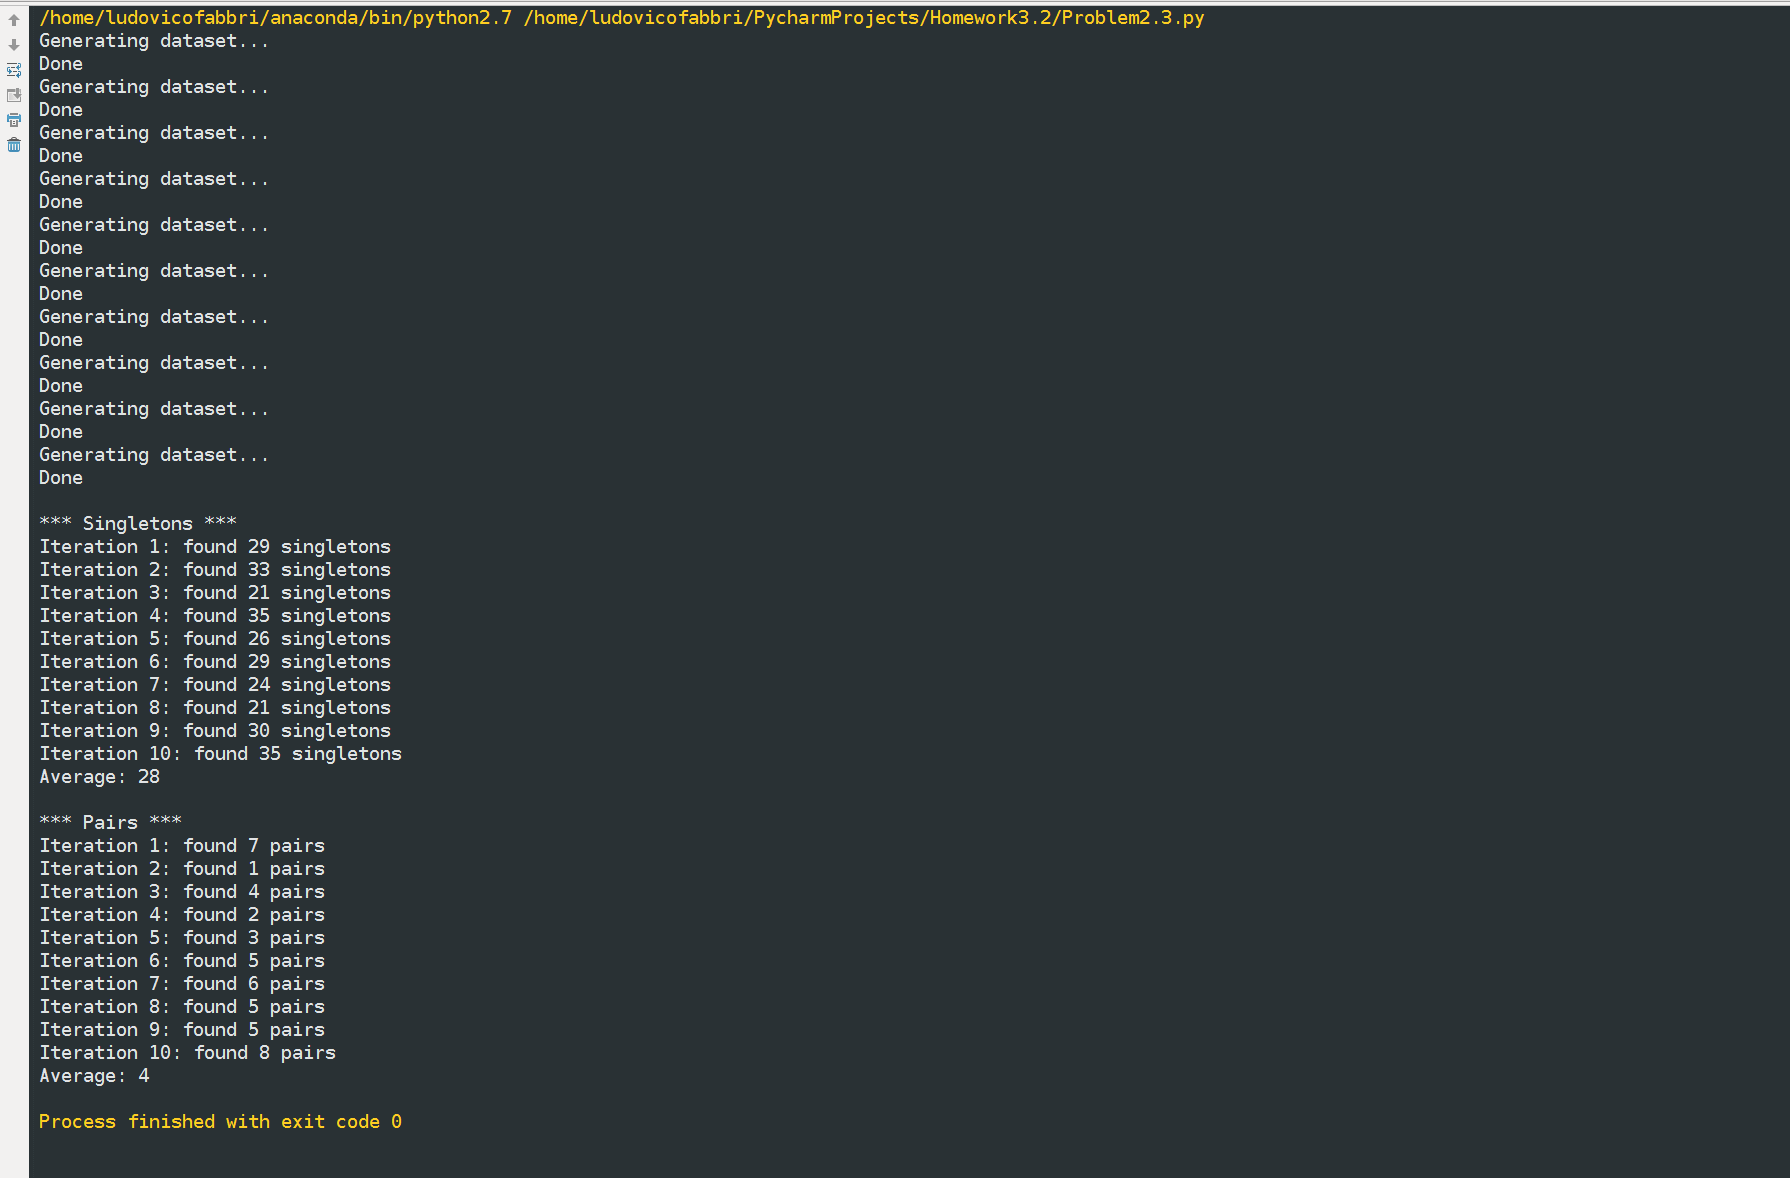
\includegraphics[width=150mm]{problem23}
\caption{Problem2.3.py  \label{problem23}}
\end{figure}





\subsection{}
How do you explain the large difference between 2 and 3 in the case of pairs? And why do we get different results for single items and pairs?

In the previous section we've done some simulations on random datasets generated using parameters of section 2.2.
We have found that the average number of singletons that have support equal or greater than 550 ($500 + 10\%(550)$) is about 28, while the average number of pairs that have support equal or greater than 12.5 ($2.5 \cdot 5$)
is about 4. From the point 2.2 we also know that the expected value to see a particular item is 500, while the expected value to see a particular pair is 2.5.

If we do some simulations on frequent singletons for a threshold that is just twice the expected value of 500 we are going to find 0 frequent items, while for pairs we see that there are few that have support greater than 5 times the expected value of 2.5. Why is there this difference?

The first thing to notice is that there much more possible pairs than singletons. In fact for  a dataset of n=2000 items we have ${2000 \choose 2} = 1999000$ possible pairs.

We can define two events:

\begin{itemize}
	\item X = "number of times a particular singleton appears"
	\item Y = "number of times a particular pair appears"	
\end{itemize}

We can think the event "singleton/pair appears more than x times" as a Bernoulli trial, so the experiment can just succeeds or fails.
From the binomial distribution we know that to get exactly k success in n trials we have:

\begin{equation} {\label{eq:binomialDistribution}}
Pr(X = k) = {n \choose k} p^k (1-p)^{n-k}
\end{equation}

where $p^k$ are the successes and $(1-p)^{n-k}$ are the failures and ${n \choose k}$ are all the possible ways of distributing k successes in a sequence of n trials.

Now we are interested in the union of events where we get exactly k successes, k+1 successes, k+2 successes and so on; the trials are the number of baskets (m=100000) and
because these are independent events we can just sum them and find:

\begin{equation} {\label{eq:probx}}
Pr(X \geq k) = \sum_{k=550}^{m} {m \choose k} p^k (1-p)^{m-k}
\end{equation}

\begin{equation} {\label{eq:proby}}
Pr(Y \geq k) = \sum_{k=13}^{m} {m \choose k} p^{2k} (1-p)^{m-2k}
\end{equation}

where $p=p^2$ in case of pairs, 550 is the 110\% of the expected value for a singleton and 13 is the integer approximation of 5 times the expected value of a pair.
Now let's compute the expected value for both the events $(X \geq k)$ and $(Y \geq k)$:

$$\mathbb{E} \left[ X \right] = n \cdot Pr(X >= k)$$

$$\mathbb{E} \left[ Y \right] = n \cdot Pr(Y >= k)$$

For singletons we have that $n=2000, \; p=0.005, \; m=10^5 \; and \; k=550$, while for pairs we have that $n={2000 \choose 2}, \; p=0.005, \; m=10^5 \; and \; k=13$, 
so we can just substitute the values in the equations and find:


\begin{equation} {\label{eq:expectedx}}
\mathbb{E} \left[ X \right] = 2000 \cdot \sum_{k=550}^{100000} {100000 \choose k} 0.005^k (1-0.005)^{100000-k} \cong 28.413
\end{equation}

\begin{equation} {\label{eq:expectedx}}
\mathbb{E} \left[ Y \right] = {2000 \choose 2} \cdot \sum_{k=13}^{100000} {100000 \choose k} 0.005^{2k} (1-0.005)^{100000-2k} \cong 4.76359
\end{equation}

As we can see we have got values that are very close to the average results in the simulations did in point 2.3, so we have mathematically prove that the results of the simulations are coherents.
Intuitively we can say that with the growing of the itemset size (from singleton to pair) we observe a decrease of the average frequency (the expected value of occurrences of the itemset which is
500 for singletons and 2.5 for pairs) and an increase of the variance, where for variance we intend the divergence from the expected value for that particular itemset. For example if we compute the expected value for 
triplets we find that it is about $0.0125$ so in theory we doesn't expect to see any frequent triplet, but they appear; the variance in this case is much larger than pairs, about 100 and much more, and we are not going
to find any frequent pair with a threshold of 100 times of the expected value of a pair. The same behavior if we increase the dimension of the itemset to 4, 5 and so on, the variance is going to explode with some exponential behavior,
while the expected value is going to decrease exponentially as well.







\section{Extra credit}
Even though the data were generated completely at random, some pairs appear to be much more frequent than others. This example shows us that we should be careful not to draw fast conclusions. Generally, often we may think that there is some signal in our data, when in reality there is none. Propose and implement a way to deal with the problem above.

One interesting and useful analysis in the study of frequent items pattern is the topic of the association rules.
An association rule is defined as $I \rightarrow j$, and tell us that if a basket contains $I$, where $I$ is a generic set of items, is likely to contains also j.
The notion of 'likely' is called \textit{confidence} of the association rule and can be formally defined as below:

$$ conf(I \rightarrow j) = \frac {support(I \cup \left\{ j \right\})} {support(I)}  $$

From the confidence we can define the notion of the \textit{interest} of the association rule, that is the difference between its confidence and the fraction of baskets of the dataset that contains j:

$$  int(I \rightarrow j) =  \frac {support(I \cup \left\{ j \right\})} {support(I)} - \frac{support(\left\{ j \right\})} {|baskets|} $$

The interest is an important indicator in the frequent pattern analysis, and tell us how much the items in the left side of the relation have influence on the items on the right side. 
For example in the relation $(pasta \rightarrow tomato)$ we expect to see an high interest (indicating that if a person buy pasta is likely to buy also tomato), while for a relation like
$(car \rightarrow cheese)$ is going to be low interest, because there is not any relationship between car and cheese. Interest could be also a negative value, indicating that the presence of $I$
discourages the presence of $j$.

For our random generated dataset used in the previous sections we expect to see very low interests between frequent itemsets, because there are no correlation between items in the baskets since they
are generated randomly.
I've wrote a python file \textit{InterestPairs.py} where i have implemented a static method to compute the interest values for the frequent pairs we found with simple apriori alghorithm.
Here is the output for the random generated dataset:

\newpage

\begin{figure} [h]
\centering
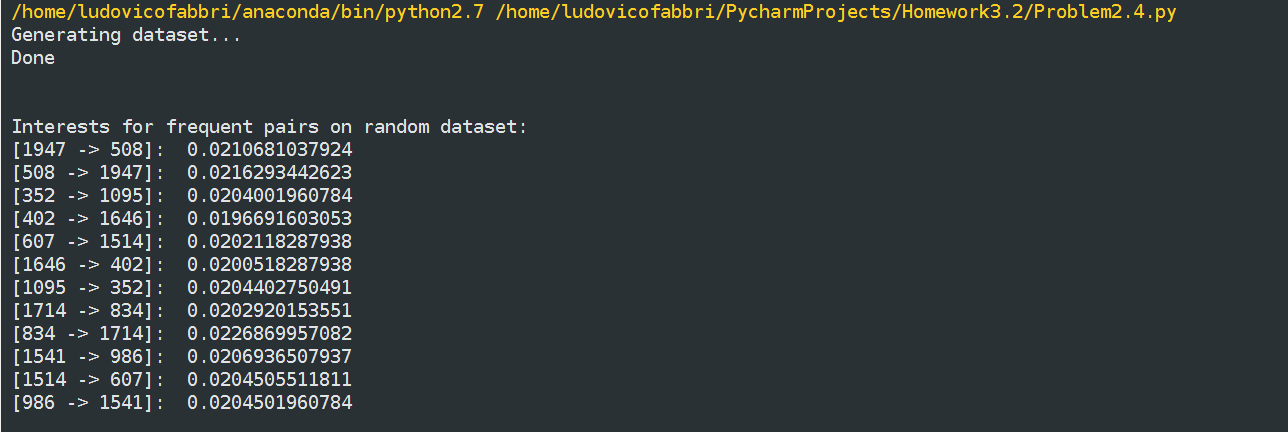
\includegraphics[width=150mm]{interestsRandom}
\caption{interests of frequent pairs for random dataset  \label{interestsRandom}}
\end{figure}


As we can see they are close to 0 and uniformly distribuited, indicating that in a random dataset is unlikely to see any relationship between frequent itemsets, as we expected.

Now let's compute the interest values for frequent pairs found after a run of simple Apriori on \textit{retail.dat} file. Below there is a portion of the output:

\begin{figure} 
\centering
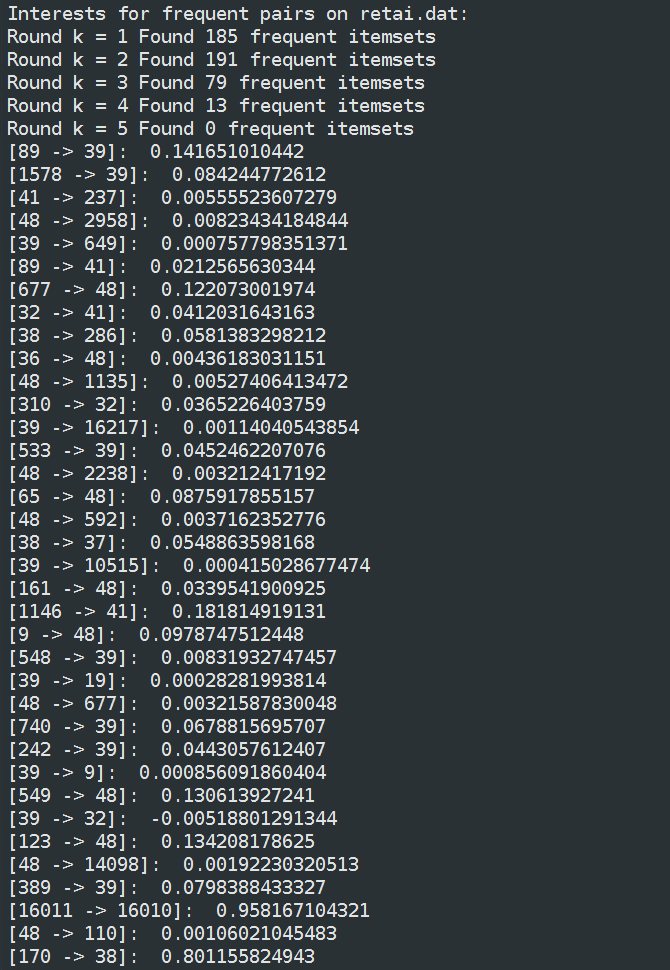
\includegraphics[width=150mm]{interestsRetail}
\caption{interests of frequent pairs on retail.dat  \label{interestsRetail}}
\end{figure}

\newpage

As we can see there is effectively some signal in data, some interests are much greater than 0. For example the association rule $170 \rightarrow 38$ has an interest of 0.8, meaning there is
a strong relationship between 170-th item and 38-th item, so a seller can know that many people that buy the 170-th item are going to buy also the 38-th item.
So in the end this type of analysis makes sense only if we are analyzing a real dataset where there are real relationships between the items of the transactions (baskets), in other cases like
using a random generated dataset this approach can't give us any useful information.
















































\end{document}


